\documentclass[onecolumn, aps, nofootinbib, prd, preprint, floats, floatfix, amsmath, amssymb, superscriptaddress, preprintnumbers]{revtex4-1}
\PassOptionsToPackage{dvipsnames}{xcolor}
\usepackage{slashed}
\usepackage{graphicx}
\usepackage{subcaption}
\usepackage{dcolumn}
\usepackage{bm}
\usepackage{amssymb}
\usepackage{tikz-feynman}
%\usepackage{xcolor}
\usepackage[utf8]{inputenc}
% \usepackage[OT1]{fontenc}
\usepackage{yfonts,amsmath,amsthm,amsfonts,amssymb,amscd, ulem}
\usepackage{enumerate}
\usepackage{fancyhdr}
\usepackage{mathtools}
\usepackage{amsmath}
\usepackage{autobreak}
\usepackage{mathrsfs}
\usepackage{cancel}
\usepackage{slashed}
\usepackage{bigints}
\usepackage[flushleft]{threeparttable}
\usepackage[colorlinks=true, citecolor=purple, linkcolor=blue]{hyperref}
\usepackage{url}
\usepackage{makecell,booktabs}
\usepackage{braket}
\usepackage{relsize}
\usepackage{multirow}
\usepackage{verbatim}
\usepackage{txfonts}
\usepackage{slashed}
\usepackage{upgreek}
\usepackage{extarrows}
\usepackage{array}
\usepackage{appendix}
\usepackage[T1]{fontenc}
\usepackage{setspace}
\usepackage{subcaption}
\newcommand{\GJH}[1]{\textcolor{blue} {GJH: #1}}
\newcommand{\jl}[1]{\textcolor{orange} {jl: #1}}
\newcommand{\WXP}[1]{\textcolor{purple} {WXP: #1}}
\newcommand{\zb}[1]{{\color{blue} {#1}}}
\usepackage{xcolor}
\definecolor{c1}{HTML}{1bd1a5}
\newcommand{\pch}[1]{\textcolor{c1} {PCH: #1}}
\usepackage{graphicx}   % 引入图片
\usepackage{caption}    % 总 caption 支持
\usepackage{subcaption} % 子图支持
\usepackage{subcaption}
\usepackage{cleveref}
\captionsetup{justification=raggedright, singlelinecheck=false}


\begin{document}

\title{An Axial $U_A(1)_{L_\mu-L_\tau}$ Gauge Boson: UV Completion and Experimental Searches}
\author{Jia Liu}
\date{May 2026}


\maketitle
\tableofcontents

\section{Introduction}

\section{Model Setup}
\label{sec:model-setup}
To construct a UV-complete axial vector ${ U_A(1)}_{L_\mu-L_\tau}$ model, we extend the SM gauge group with an additional ${ U_A(1)}_{L_\mu-L_\tau}$ gauge group. Additionally, we introduce two new vector-like leptons $E_\mu$, $E_\tau$, and a complex scalar $S$, both of which are singlets under the SM group but charged under the ${U_A(1)}_{L_\mu-L_\tau}$ gauge group. The gauge charges of these particles are summarized in Tab. \ref{tab:charge-assignment}, which can ensure that the triangle anomalies cancel exactly between the $\mu$ and $\tau$ sectors, even if each generation is individually chiral under this new axial vector group. For example, including the $SU(2)_L$ multiplicity and subtracting the right-handed contribution, $\mathcal{A}_{[U_A(1)'_{L_\mu-L_\tau}]^3} \propto 2(+1)^3-(-1)^3+2(-1)^3-(+1)^3=0$, and the mixed gravitational anomaly cancels in the same way. Besides, this ${U_A(1)}_{L_\mu-L_\tau}$ symmetry can be broken by the newly introduced $S$, which can supply the charge insertion needed to generate the SM charged-lepton masses.
\begin{table}[htbp]
    \centering
    \begin{tabular}{cccc}
    \hline
    Field & $SU(2)_L$ & $U(1)_Y$ & $U_A(1)'_{L_\mu-L_\tau}$ \\
    \hline
    $L_{\mu}=\left(\nu_{\mu}, \mu_L\right)^T$ & $\mathbf{2}$ & $-1 / 2$ & $Q_{\ell}$ \\
    \hline
    $\mu_R$ & $\mathbf{1}$ & -1 & $-Q_\ell$ \\
    \hline
    $E_\mu\left(E_{\mu L}, E_{\mu R}\right)$ & $\mathbf{1}$ & -1 & $Q_\ell$\\
    \hline
    $L_{\tau}=\left(\nu_{\tau}, \tau_L\right)^T$ & $\mathbf{2}$ & $-1 / 2$ & $-Q_\ell$ \\
    \hline
    $\tau_R$ & $\mathbf{1}$ & -1 & $Q_\ell$ \\
    \hline
    $E_\tau\left(E_{\tau L}, E_{\tau R}\right)$ & $\mathbf{1}$ & -1 & -$Q_\ell$\\
    \hline
    $H$ & $\mathbf{2}$ & $1 / 2$ & 0 \\
    $S$ & $\mathbf{1}$ & 0 & $Q_S=2Q_\ell$\\
    \hline
    \end{tabular}
    \caption{Field content and \(U_A(1)'_{L_\mu-L_\tau}\) charge assignment for the axial \(L_\mu-L_\tau\) construction. The electron sector is neutral under \(U_A(1)'_{L_\mu-L_\tau}\).}
    \label{tab:charge-assignment}
\end{table}

Based on the charges of the particles under the gauge groups, the relevant Lagrangian can be expressed as
\begin{equation}\label{eq:Lagrangian}
\begin{aligned}
\mathcal{L}_{UV}\supset& -\frac{1}{4}A'_{\alpha\beta}A'^{\alpha\beta}+\sum_{\alpha=\mu,\tau}\left(i\bar{L}_\alpha \gamma^\nu D_{\nu} L_\alpha + i\bar{\ell}_{\alpha R} \gamma^\nu D_{\nu}\ell_{\alpha R} + i\bar{E}_{\alpha}\gamma^\nu D_{\nu} E_{\alpha}\right)  \\
&+\sum_{\alpha=\mu,\tau}\left(-y_\alpha \bar L_\alpha H E_{\alpha R} -\lambda_\alpha S^{(*)}\bar E_{\alpha L}\ell_{\alpha R} -M_{E\alpha}\bar E_{\alpha L}E_{\alpha R} + h.c.\right)\\
&+ (D_{\nu}S)^\dagger (D^{\nu}S) - V(S),
\end{aligned}
\end{equation}
where $A'_{\alpha\beta}=\partial_\alpha A'_\beta - \partial_\beta A'_\alpha$ is the field-strength tensor, the covariant derivative is given by $D_\nu = \partial_\nu -ig_Y \frac{Y}{2}B_\nu  -ig_W T^iW_\nu^i - ig_{A'} Q_{A'} A'_\nu$, where $B_\nu$, $W_\nu^i$ and $A'_\nu$ represent the gauge fields for the ${U(1)}_Y$, ${SU(2)}_L$ and ${U_A(1)}_{L_\mu-L_\tau}$ groups, respectively. The constants $g_Y$, $g_W$ and $g_{A'}$ are their associated coupling constants. And, $V(S)$ is the self-interacting potential of $S$. Furthermore, the ordinary diagonal SM Yukawa operator $\bar L_\ell H\ell_R$ is forbidden due to the charge assignment. Consequently, the interactions between charged leptons and Higgs in this model necessarily arise via the new fields, $E$ and $S$. Integrating out the heavy field $E$ at the matching scale $\lambda=M_E$ generates the following dimension-5 effective operators:
\begin{equation}\label{eq:5-d}
    \mathcal{L}_{\text{5-d}} =
    -\frac{c_\mu}{\Lambda} S \bar{L}_\mu H\mu_R
    -\frac{c_\tau}{\Lambda} S^* \bar{L}_\tau H\tau_R
    +h.c.,
\end{equation}
where, in the tree level, $\frac{c_\alpha}{\Lambda}\simeq \frac{y_\alpha \lambda_\alpha}{M_{E\alpha }}$ for $\alpha=\mu,\tau$.

After the electroweak and $U_A(1)_{L_\mu-L_\tau}$ spontaneous symmetry breaking, the scalar fields are given by $H=\frac{1}{\sqrt{2}}\left (\begin{array}{c} 0 \\ v_h+h \end{array}\right)$ and $S=\frac{1}{\sqrt{2}} (v_s + s)$, where $v_{h/s}$ denotes the vacuum expectation value (vev) of the Higgs and scalar $S$, respectively. Then, the $A'$ mass follows from $(D_{\nu}S)^\dagger (D^{\nu}S)$, $m_{A'} = |Q_S| g_{A'} v_s = 2 |Q_\ell| g_{A'} v_s \equiv 2|g_X|v_s$ with $g_X\equiv g_{A'} Q_\ell$. And the mass terms for leptons can be derived as
\begin{equation}
\mathcal{L}_{\mathcal M}=-
\begin{pmatrix}
	\overline{\ell^{\mu}_L},  &
	\overline{E^\mu_L}, &
	\overline{\ell^\tau_L}, &
	\overline{E^\tau_L}
\end{pmatrix}
\begin{pmatrix}
	0 & y_{\mu}v_h/\sqrt2  & 0 & 0 \\
	\lambda_\mu v_s/\sqrt2 & M_{E\mu} & 0 & 0\\
	0 & 0 & 0 & y_{\tau}v_h/\sqrt2\\
    0 & 0 &  \lambda_\tau v_s/\sqrt2 & M_{E\tau}
\end{pmatrix}
\begin{pmatrix}
	\ell^{\mu}_R \\
	E^\mu_R \\
	  \ell^\tau_R \\
	  E^\tau_R \\
\end{pmatrix}
+h.c. = -\bar{\chi}_L \mathcal{M} \chi_R + h.c.
\label{eq:4by4-mass-no-mutau}
\end{equation}
Here, $\chi_L=(\ell^{\mu}_L,E^\mu_L,\ell^\tau_L, E^\tau_L)^T$, $\chi_R=(\ell^{\mu}_R,E^\mu_R,\ell^\tau_R, E^\tau_R)^T$.
And the $4\times 4$ mass matrix $\mathcal{M}$ exhibits a block structure, so it can be block-diagonalized via the seesaw-like diagonalization procedure. For the muon block, we can reorganize its mass term as
\begin{equation}
\mathcal{L}_{\mathcal{M},\mu}
=-\overline{\chi^\mu_L}\,\mathcal{M}_\mu\,\chi^\mu_R+h.c.,
\qquad
\mathcal{M}_\mu =
\begin{pmatrix}
0 & m_L\\
m_R & M_{E\mu}
\end{pmatrix},
\label{eq:mu-2by2-mass}
\end{equation}
with $\chi^\mu_L=(\ell^\mu_L, E^\mu_L)^T$, $\chi^\mu_R =
(\ell^\mu_R,E^\mu_R)^T$, and $m_L=\frac{y_\mu v}{\sqrt2},
m_R=\frac{\lambda_\mu v_s}{\sqrt2}$. Assuming these mass entries are real, the mass matrix can be bi-orthogonally diagonalized as
\begin{equation}
U_{\mu L}^T\mathcal{M}_\mu U_{\mu R} =
\begin{pmatrix}
m_\mu &0\\
0&m_{E\mu}
\end{pmatrix},~ {\rm with}~
\chi^\mu_L=U_{\mu L} \chi^{\mu \prime}_L~{\rm and}~
\chi^\mu_R=U_{\mu R} \chi^{\mu \prime}_R,
\end{equation}
with $U_{\mu L/\mu R}=\begin{pmatrix}\cos\theta_{\mu L/\mu R} &\sin\theta_{\mu L/\mu R}\\-\sin\theta_{\mu L/\mu R} & \cos\theta_{\mu L/\mu R} \end{pmatrix}$. And the mass eigenvalues are
\begin{equation}
m_{\mu/E\mu}^2=
\frac{1}{2}
\left[
m_L^2+m_R^2+M_{E\mu}^2 \mp
\sqrt{(m_L^2+m_R^2+M_{E\mu}^2)^2-4m_L^2m_R^2}
\right].
\label{eq:exact-masses-2by2}
\end{equation}
The mixing angles can be written as
\begin{equation}
\tan2\theta_{\mu L}= \frac{2m_L M_{E\mu}}{M_{E\mu}^2+m_R^2-m_L^2},
\qquad
\tan2\theta_{\mu R}=\frac{2m_R M_{E\mu}}{m_L^2+M_{E\mu}^2-m_R^2}.
\label{eq:mixing-angles-2by2}
\end{equation}
In the limit $M_{E\mu}\gg m_L, m_R$, to the leading order, the muon block masses and mixing angles can be simplified to
\begin{equation}
\begin{aligned}
    &m_\mu^2\simeq\frac{m_L^2 m_R^2}{M_{E\mu}^2},~ m_{E\mu}^2\simeq M_{E\mu}^2+(m_L^2 + m_R^2)\\
    &\theta_{\mu L}\simeq \frac{m_L}{M_{E\mu}},~ \theta_{\mu R}\simeq \frac{m_R}{M_{E\mu}},
\end{aligned}
\end{equation}
where the mass terms are consistent with the ones in 5-d effective operators in Eq. \eqref{eq:5-d} after the symmetry breaking. 

Next, we will consider the Lagrangian in the mass eigenstates. We can decompose the interaction into two parts: gauge interaction and scalar interaction,
\begin{equation}
    \mathcal{L}_{\rm int}\supset \mathcal{L}_{\rm gauge} + \mathcal{L}_{\rm scalar}.
\end{equation}
The relevant gauge Lagrangian part can be expanded as
\begin{equation}
\begin{aligned}
\mathcal{L}_{\rm gauge}
&\supset~
\overline{\chi^{\mu\prime}_L}\gamma^\alpha
\bigg[-eA_\alpha\,\mathbf{1}+g_X A'_\alpha\,\mathbf{1} +Z_\alpha
\begin{pmatrix}
g_{\ell_L}^Z c_L^2+g_E^Z s_L^2 & (g_{\ell_L}^Z-g_E^Z)c_Ls_L\\
(g_{\ell_L}^Z-g_E^Z)c_Ls_L & g_{\ell_L}^Z s_L^2+g_E^Z c_L^2
\end{pmatrix}
\bigg] \chi^{\mu\prime}_L,\\
&+~\overline{\chi^{\mu\prime}_R}\gamma^\alpha
\bigg[ -eA_\alpha\,\mathbf{1} +g_E^ZZ_\alpha\,\mathbf{1} -g_XA'_\alpha
\begin{pmatrix}
\cos2\theta_{\mu R} & \sin2\theta_{\mu R}\\
\sin2\theta_{\mu R} & -\cos2\theta_{\mu R}
\end{pmatrix}\bigg]\chi^{\mu\prime}_R\\
&+\frac{g_W}{\sqrt2}
\left[
\bar\nu_{\mu L}\gamma^\alpha
\left(c_L\mu'_L+s_L E'_{\mu L}\right)W^+_\alpha
+h.c.
\right]\\
&+ \frac{m_{A'}^2}{v_s}s A'_\alpha A'^\alpha + \frac{m_{A'}^2}{2 v_s^2}s^2 A'^2.
\end{aligned}
\label{eq:mass-basis-NC}
\end{equation} 
where $g_Z=\sqrt{g_W^2+g_Y^2}$, $s_W=g_Y/g_Z$, $c_L=\cos\theta_L$ and $s_L=\sin\theta_L$. The neutral-current couplings of the doublet and singlet charged leptons to the SM $Z$ boson are $g_{\ell_L}^Z=g_Z\left(-\frac12+s_W^2\right), ~g_E^Z=g_Z s_W^2$. We can see that the electromagnetic coupling is unchanged because it is proportional to the identity. The left $A'$ coupling is also unchanged because $\ell_L^\mu$ and $E_L^\mu$ carry the same $U_A(1)'_{L_\mu-L_\tau}$ charge. The right $A'$ coupling is not exactly diagonal because $\ell_R^\mu$ and $E_R^\mu$ have opposite $U_A(1)'_{L_\mu-L_\tau}$ charges, but the off-diagonal coupling is suppressed by $\sin2\theta_{\mu R}\simeq 2m_R/M_{E\mu}$ in the large $M_{E\mu}$ expansion.

While for the scalar interaction part relevant to the Higgs and $s$, it can be reduced to
\begin{equation}
\begin{aligned}
\mathcal{L}_{\rm scalar} &
\supset-\overline{\chi_L^\mu}
\left[
\frac{m_L}{v_h}\,h
\begin{pmatrix}
0&1\\
0&0
\end{pmatrix}
+
\frac{m_R}{v_s}\,s
\begin{pmatrix}
0&0\\
1&0
\end{pmatrix}
\right]\chi_R^\mu
+h.c. .\\
&=-\overline{\chi'_L}
\left[\frac{m_L}{v_h} h \begin{pmatrix}
c_Ls_R&c_Lc_R\\
s_Ls_R&s_Lc_R
\end{pmatrix}+ \frac{m_R}{v_s} s \begin{pmatrix}
s_Lc_R&-s_Ls_R\\
-c_Lc_R&c_Ls_R
\end{pmatrix}\right]\chi'_R+h.c.,
\label{eq:gauge-basis-scalar-yukawa}
\end{aligned}
\end{equation}
For the light charged lepton, the diagonal couplings are therefore
\begin{equation}
y_{h\mu\mu}=
\frac{m_L}{v_h}c_Ls_R,
\qquad
y_{s\mu\mu}=\frac{m_R}{v_S}s_Lc_R .
\label{eq:light-scalar-yukawa}
\end{equation}
In the seesaw-like limit $M_E\gg m_L,m_R$, these reduce to
\begin{equation}
y_{h\mu\mu}\simeq
\frac{m_\mu}{v_h}
\qquad
y_{s\mu\mu}\simeq \frac{m_\mu}{v_s}.
\label{eq:sm-limit-scalar-yukawa}
\end{equation}
Thus, the SM muon Yukawa coupling is recovered for the observed Higgs in the combined decoupling/alignment limit $M_{E\mu}\gg m_L,m_R$, and with the singlet-like scalar either heavy or weakly mixed, which is consistent with the leading order terms in Eq. \eqref{eq:5-d} after the phase transition. Outside this limit, the new scalar interactions include the singlet coupling proportional to $m_\mu/v_s$, and scalar-mediated transitions between the light lepton and the heavy vector-like lepton.

For the light state ($\mu^\pm$) alone, the diagonal $A'$ coupling is
\begin{equation}
\mathcal{L}_{A'}^{\mu'}
=
A'_\alpha\bar\mu'\gamma^\alpha
\left[
g_X\sin^2\theta_{\mu R}
-g_X\cos^2\theta_{\mu R} \gamma_5
\right]\mu'
+\cdots .
\label{eq:light-muon-Apr}
\end{equation}
Thus, the coupling remains dominantly axial, with only an $\mathcal{O}(\theta_{\mu R}^2)$ vector admixture. The $\tau$ block is obtained by the replacements $\mu\to\tau$ and by reversing the $U_A(1)'_{L_\mu-L_\tau}$ charges.

At the UV level, the model initially contains ten independent free parameters:
\begin{equation}
    \{v_s, y_\mu, y_\tau, \lambda_\mu,\lambda_\tau, M_{E\mu}, M_{E\tau}, Q_\ell, g_{A'}, m_s \}.
    \end{equation}
After electroweak symmetry breaking and after matching to the observed muon and tau pole masses, two combinations of the UV parameters are fixed, leaving eight physically independent low-energy free parameters:
\begin{equation}
    \{v_s, \theta_{\mu L}, \theta_{\tau L}, \theta_{\mu R},\theta_{\tau R}, Q_\ell, g_{A'}, m_s \},
    \end{equation}
which satisfy the mass relations
\begin{equation}
    m_\mu\simeq \theta_{\mu L} \theta_{\mu R} M_{E\mu}, \qquad
    m_\tau\simeq \theta_{\tau L} \theta_{\tau R} M_{E\tau}.
    \end{equation}
To simplify the phenomenological analysis, we follow the previously introduced assumption that the vector-like leptons are considerably heavier than all off-diagonal lepton mass terms. We further restrict the parameter space by directly adopting the scalar mass $m_s$ from the scalar potential $V(S)$, imposing $M_{E\mu},M_{E\tau} > 10~\mathrm{TeV}$, and fixing $Q_\ell=1$. Under these simplifications, the lepton mixing angles satisfy
\begin{equation}
    \theta_{\mu L}\theta_{\mu R}\lesssim 10^{-5}, \qquad
    \theta_{\tau L}\theta_{\tau R}\lesssim 10^{-4}.
    \end{equation}
The phenomenology of the scalar singlet $s$ and vector-like leptons is subdominant and less relevant to our core analysis, for two key reasons. First, observable signatures of the scalar $s$ arise from $A'$-mediated processes or Higgs-like leptonic interactions, which are severely suppressed by the factors $m_{A'}^2/v_s$ and $m_{A'}^2/v_s^2$ or the small charged-lepton Yukawa ratios $m_{\mu/\tau}/v_s$. Second, the physics of vector-like leptons in comparable parameter regimes has already been comprehensively investigated in existing literature~\cite{Cao:2023smj,Yue:2026tbc,Yue:2025xvk,Yue:2024sds}. Combined with their large masses and the extremely suppressed lepton mixing angles derived above, these states do not yield prominent signatures for our targeted experiments. For this reason, we do not conduct dedicated searches for the scalar singlet and vector-like leptons in this work and leave their detailed phenomenological exploration for future studies. Instead, we concentrate solely on probing the axial vector boson $A'$ across the broad mass range $m_{A'}\in [\mathrm{MeV}, \mathrm{TeV}]$, which is of key interest for neutrino and muonphilic experiments. With all above simplifications, the final set of physically relevant parameters reduces to
\begin{equation}
    \{v_s, g_{A'}\} \quad \text{or} \quad \{m_{A'}, g_{A'}\}.
\end{equation}

It is worth noting that, in fact, when we consider the Lagrangian in Eq. \eqref{eq:Lagrangian}, gauge invariance also allows an off-diagonal SM-Higgs Yukawa interaction,
\begin{equation}
    \mathcal{L}\supset
    -y_{\mu\tau}(\bar{L}_{\mu}H \tau_R + \bar{L}_{\tau}H \mu_R)+h.c. .
\label{eq:ymutau-operator}
\end{equation}
When included, this term generates non-zero off-diagonal entries $\mathcal{M}_{13}=\mathcal{M}_{31}=y_{\mu\tau}v_h/\sqrt{2}$ in the lepton mass matrix of Eq.~\eqref{eq:4by4-mass-no-mutau}, which induces charged-lepton flavor violation (CLFV) at tree level. Stringent experimental limits on $y_{\mu\tau}$ have been established via measurements of CLFV processes, including $\tau\to\mu +{\rm Inv}$ \cite{Ibarra:2021xyk}, $\tau\to\mu \mu\mu$ \cite{Ibarra:2021xyk,Hayasaka:2010np,Belle-II:2024sce}, $\tau\to \mu\gamma$ \cite{Belle:2021ysv}, $h\to\mu\tau$ \cite{Harnik:2012pb,CMS:2021rsq} and $Z\to \mu\tau$ \cite{ATLAS:2021bdj}.
A systematic overview of CLFV phenomenology in the tau sector is provided in Ref.~\cite{Banerjee:2022xuw}. Given these strong bounds, we adopt $y_{\mu\tau}=0$ as our benchmark scenario in this work.

Notably, a vanishing $y_{\mu\tau}=0$ need not be a purely numerical accident. It can be naturally realized if the charged-lepton sector respects an approximate $U(1)_{F_\mu}\times U(1)_{F_\tau}$, or a discrete subgroup, under which $(L_\ell,\ell_R,E_{\ell L},E_{\ell R})$ carry a common family label while $H$ and $S$ are neutral. In this framework, the diagonal Yukawa chains in Eq.~\eqref{eq:Lagrangian} preserve the family number, whereas the off-diagonal operator in Eq.~\eqref{eq:ymutau-operator} explicitly breaks it. Motivated both by the tight experimental constraints and by the natural flavor-symmetric structure described above, we take $y_{\mu\tau}$ as a simplifying assumption throughout our analysis.

\section{Existing Constraints}
\label{sec:phenomenology}
As demonstrated above, we mainly focus on the exploration of axial vector boson. In the limits of tiny mixing angles, heavy vector-like leptons and new scalar, the most relevant Lagrangian can be reorganized and reduced to
\begin{equation}
\begin{aligned}
\mathcal{L}_{A'} \supset & -g_XA'_\alpha\bar\mu\gamma^\alpha\gamma^5\mu
+g_XA'_\alpha\bar\nu_\mu\gamma^\alpha P_L\nu_\mu \\
&+g_X A'_\alpha\bar\tau\gamma^\alpha\gamma^5\tau - g_X A'_\alpha\bar\nu_\tau\gamma^\alpha P_L\nu_\tau,
\end{aligned}
\label{eq:phenomenology-coupling-convention}
\end{equation}
with $g_X\equiv g_{A'} Q_\ell$. The small vector admixture induced by vector-like lepton mixing is given in Eq.~\eqref{eq:light-muon-Apr}; unless stated otherwise, the phenomenological limits below are quoted in the pure-axial limit. In this limit, the most relevant existing constraints come from the neutrino trident process, muon beam-dump searches, invisible pion decays, and muon $g-2$. 

\subsection{Neutrino Trident Production}
\label{subsec:trident}

Neutrino trident production is the most direct low-energy probe of the interaction pattern in our model, which has been searched for in several neutrino beam experiments, such as the CHARM II collaboration \cite{geiregat1990first} and the CCFR collaboration \cite{CCFR:1991lpl}. According to their reported results, we have 
\begin{equation}
\begin{aligned}
\sigma_{\mathrm{CHARM}-\mathrm{II}} / \sigma_{\mathrm{SM}} & =1.58 \pm 0.57 \\
\sigma_{\mathrm{CCFR}} / \sigma_{\mathrm{SM}} & =0.82 \pm 0.28.
\end{aligned}
\end{equation}
These results strongly constrain our model.
Following the equivalent-photon treatment of Refs. \cite{Williams:1934ad,Belusevic:1987cw,Altmannshofer:2014pba}, the nuclear cross section for $\nu_\mu N\to \nu_\mu N\mu^+\mu^-$ can be obtained by folding the real-photon subprocess with the photon flux of the target nucleus,
\begin{equation}
\sigma(\nu_\mu N\to\nu_\mu N\mu^+\mu^-)
=\int ds\,dq^2\,
\frac{Z^2\alpha}{\pi}\frac{F^2(q^2)}{s\,q^2}\,
\sigma(\nu_\mu\gamma\to\nu_\mu\mu^+\mu^-),
\label{eq:trident-epa}
\end{equation}
where $Ze$ and $F(q^2)$ are the charge and the electromagnetic form-factor of the nucleus, respectively (see Ref. \cite{Altmannshofer:2014pba} for more details).
For analytic intuition, if terms proportional to the muon mass are dropped, after careful calculation, we find that the result of $\sigma(\nu_\mu\gamma\to\nu_\mu\mu^+\mu^-)$ has a similar structure to Eq.~(7) in Ref.~\cite{Altmannshofer:2014pba} but with a shift on $C_{\rm A}$ instead of $C_{\rm V}$ in vector case.
And the full square of the matrix element for this $\nu_\mu\gamma\to\nu_\mu\mu^+\mu^-$ process can be approximately as
\begin{equation}
\begin{aligned}
\frac{1}{2} \sum_{\mathrm{pol}}\left|M_1 M_2\right|^2=512\left|\mathcal{M}_{\mathrm{V}-\mathrm{A}}\right|^2 \times \frac{1}{2}\left[C_{\mathrm{V}}^2+\left(C_{\mathrm{A}}-\frac{g_X^2}{\sqrt2G_F}\,
\frac{1}{k^2-m_{A'}^2}\right)^2 \right].
\end{aligned}
\end{equation}
Here, $k$ is the momentum of the exchanged $A'$ and the SM coefficients of the vector and axial-vector currents in the interaction of muon-neutrinos with muons are $C_{\mathrm{V}}=\frac{1}{2}+ 2 \sin ^2 \theta_{\mathrm{w}}, C_{\mathrm{A}}=\frac{1}{2}$, with $\theta_{\mathrm{w}}$ being the weak mixing angle. Then, after the phase-space integration, the total cross section can be obtained. In the heavy mass limit of $m_{A'}\gg\sqrt{s}$, the total cross section to SM cross section can be expressed as
\begin{equation}
    \frac{\sigma^{\rm SM+A'}}{\sigma^{\rm SM}}\simeq\frac{C_V^2+[C_A+g_X^2/(\sqrt{2}G_F m_{A'}^2)]^2}{C_V^2+C_A^2}.
\end{equation}
For moderate or light $A'$, the exact phase space integration and consideration of muon mass must be included. However, to the leading order of new physics, we can do the substitution $C_{\rm V} C_{\rm V}^{(Z')}\to C_{\rm A}\cdot \frac{g_X^2}{\sqrt2G_F}$ to obtain the constraints on $g_X-m_{A'}$ where $C_{V}^{(Z')}=\frac{v_h^2}{m_{Z'}^2/g'^2}$ and the constraint on $g'-m_{Z'}$ is extracted from Fig. 2 in Ref. \cite{Altmannshofer:2014pba}.
In fact, for the actual constraint, we do not use the massless analytic expression or the simple substitution. Instead, we evaluate the full spin- and polarization-summed Bethe-Heitler amplitude for $\nu_\mu\gamma\to\nu_\mu\mu^+\mu^-$, keep the finite muon mass, and perform a Monte-Carlo integration of the three-body phase space inside the EPA convolution. The results are shown in Fig. \ref{fig:allconstraints}.

\subsection{Invisible Pion Decays}
\label{subsec:pion-invisible}

Stopped-pion experiments provide an additional low-mass handle on the same axial interaction. Ref. \cite{Altmannshofer:2026opc} gave a thorough study on the invisible three-body decays, $\pi^+\to \ell^+\nu_\ell X$, for a scalar or vector $X$. And it also recast the PIENU search \cite{PIENU:2021clt} while projecting the reach of PIONEER \cite{PIONEER:2022yag,PIONEER:2022alm}. For the present analysis, we adopt existing results from the PIENU experiment to place constraints on our model, while neglecting prospective bounds from the upcoming PIONEER experiment for now. For this $U_A(1)_{L_\mu-L_\tau}$ model, the most relevant channel is
\begin{equation}
    \pi^+\to \mu^+ \nu_\mu +A'
\end{equation}
with $A'$ radiated off the external muon and muon neutrino legs, which is open only for $m_{A'}<m_{\pi^+}-m_\mu\simeq33.9~{\rm MeV}$. As to the electron channel considered in Ref. \cite{Altmannshofer:2026opc}, it is absent at tree level in our model, up to the loop-induced kinetic mixing generated by the $\mu$ and $\tau$ currents. Besides, now that $m_{A'}\simeq33.9~{\rm MeV}$, the tree-level charged muon mode is closed, while the neutrino channels remain open, which is significantly more dominant than the possible $A'\to e^+e^-$ (if $m_{A'}\gtrsim 2m_e$) generated by loop-induced kinetic mixing across the pion-decay mass window. Thus, we can take $A'$ invisible for the whole parameter space considered here.


For our pure-axial benchmark, the normalized differential rate can be written as \cite{Altmannshofer:2026opc}
\begin{equation}\label{eq:pion-axial-spectrum}
\begin{aligned}
\frac{d{\rm BR}(\pi^+\to\mu^+\nu_\mu A')}
{{\rm BR}(\pi^+\to\mu^+\nu_\mu)}
&=\frac{g_X^2}{2\pi^2}\,
\frac{dE_\mu dE_{A'}}{m_\pi^2}\,
\frac{1}{(1-x_\mu)^2}\cdot \left[\frac{x_{\mu A'}+2-3 x_{\mu}}{x_{\nu A'}}-\frac{2\left(x_{\mu A'}-1+x_{\nu A'}\right)}{x_{A'}}-\frac{\left(1-x_{\mu}\right) x_{A'}}{x_{\nu A'}^2}\right.\\
& \left. +\frac{2 x_{\mu}}{x_{\mu A'}-x_{\mu}}\left(\frac{x_{A'}}{x_{\nu A'}}-\frac{x_{\nu A'}}{x_{A'}}\right) -\frac{2\left(1-x_{\mu}\right)^2}{\left(x_{\mu A'}-x_{\mu}\right) x_{\nu A'}}+\frac{2+x_{\nu A'}-6 x_{\mu}}{x_{\mu A'}-x_{\mu}}-\frac{\left(1-x_{\mu}\right)\left(x_{A'}-4 x_{\mu}\right)}{\left(x_{\mu A'}-x_{\mu}\right)^2}\right],
\end{aligned}
\end{equation}
where $x_{\mu/A'}=m_{\mu/A'}^2/m_\pi^2$, and $x_{a b}=\frac{(p_a+p_b)^2}{m_\pi^2}$, given by Ref. \cite{Altmannshofer:2026opc}. This spectrum distorts the low-energy tail of the muon kinetic-energy distribution rather than producing a narrow line. Consequently, the bound is obtained by fitting a continuous signal shape to the PIENU muon-energy spectrum. Following the procedure in Ref. \cite{Altmannshofer:2026opc}, the limit of invisible three-body decay, $\pi^+\to\mu^+\nu_\mu A'$, measured by PIENU, can be derived as shown in Fig. \ref{fig:allconstraints}.
We can see that present PIENU data exclude roughly $g_X\gtrsim{\rm few}\times10^{-3}$ at MeV masses, weakening to $\mathcal O(10^{-1})$ as $m_{A'}$ approaches the pion-decay endpoint.

\subsection{Muon Beam-Dump Searches}
\label{subsec:muon-beam-dump}

Complementary to neutrino trident production, muon beam-dump experiments also provide a direct probe of the charged-muon interaction. Ref.~\cite{Chakraborty:2025jbd} studied the present and future sensitivity of NA64$_\mu$ \cite{NA64:2024nwj}, M$^3$ \cite{Kahn:2018cqs}, MuSIC \cite{Acosta:2021qpx,Acosta:2022ejc}, and a future muon beam dump to the vector $U(1)_{L_\mu-L_\tau}$ gauge boson \cite{Cesarotti:2022ttv}. Back to our axial $U(1)_{L_\mu-L_\tau}$ interaction, here we take the existing NA64$_\mu$ searches as the example to obtain the constraints by following a similar procedure as Ref.~\cite{Chakraborty:2025jbd}.
For kinematic allowable $A'$, the most relevant production channel is
\begin{equation}
\mu^- A(\text{Pb}) \to \mu^- A(\text{Pb}) A', \quad A' \to \text{invisible}
\label{eq:NA64production}
\end{equation}
where the target is made of lead (Pb) \cite{andreev2024exploration} and the new axial vector is emitted from the incoming or outgoing muon line. 
Keeping the muon mass terms, the axial cross section of the Bremsstrahlung is \cite{Chakraborty:2025jbd}
\begin{equation}
\begin{aligned}
\frac{d\sigma^{A'}_{2\to 3}}{dx}
&=\frac{\alpha^2\chi\,\beta\,g_X^2 x}{3\pi m_{A'}^2\left[m_{A'}^2(1-x)+m_\mu^2x^2\right]^2} \\
&\times\left[ 6m_\mu^4x^4 -2m_{A'}^4(x-1)\{x(x-3)+3\} +m_\mu^2m_{A'}^2x^2(x-4)(3x-4) \right],
\label{eq:beamdump-axial-spectrum}
\end{aligned}
\end{equation}
where $x=E_{A'}/E_\mu$, $\chi$ is the effective photon flux of the target, and $\beta$ is the final-state velocity factor [for more details, see Ref. \cite{Chakraborty:2025jbd}].
And this axial production rate coincides with the vector one in the formal $m_\mu\to0$ limit. At low $m_{A'}$, the nonconservation of the axial current enhances longitudinal $A'$ emission, and the production rate scales roughly like $m_\mu^2/m_{A'}^2$ relative to the vector benchmark.

With the differential cross section, the expected number of signal events corresponding to invisible decays of the form $A' \to \nu\bar{\nu}$ at the NA64$\mu$ experiment can be expressed as
\begin{equation}
N_{\text{sig}} = \frac{N_{\text{MOT}} n_{\text{Pb}}}{\langle dE_\mu/dy \rangle} \int_{E_{\mu,\min}}^{E_{\mu,\max}} dE_0 \int_{x_{\min}}^{x_{\max}} dx \frac{d\sigma_{2\to3}^{A'}}{dx} Br(A' \to \bar{\nu}\nu) N(m_{A'})
\label{eq:NA64Signal}
\end{equation}
where $N_{\text{MOT}}$ is the total number of muons on target, $Br(A'\to\bar{\nu}\nu)$ represents the invisible branching ratio of $A'$, $n_{\text{Pb}}$ denotes the number density of lead nuclei in the target, and $\langle dE_\mu/dy\rangle$ represents the average energy loss per unit length for muons traversing the lead target, which is assumed to be constant \cite{navas2024review}. And $N(m_{A'})$ is a normalization factor treated as a function of the $A'$ mass, which accounts for background normalization and has been calibrated using the 4D results reported by the NA64$_\mu$ experimental analysis (given in Fig.~3 of Ref. \cite{andreev2024exploration}) for the current bound corresponding to $\mathrm{N_{MOT}} \approx 2 \times 10^{10}$. And the integration bounds adopted in this function are taken from Ref. \cite{Chakraborty:2025jbd}; further details can be found in Sec. III and IV of Ref. \cite{Chakraborty:2025jbd}. With this setup, we can compute the expected number of signal events, which we then use to derive model constraints. Precisely speaking, a 90\% confidence level exclusion limit is conventionally set by requiring $N_{\text{sig}} > 2.3$ across the $(m_{A'}, g_X)$ parameter plane. In practice, Ref. \cite{Chakraborty:2025jbd} already presents exclusion limits for the vector $U(1)_{L_\mu-L_\tau}$ parameter space. Since the detector configuration and search strategy are identical between the two analyses, we can straightforwardly extract the corresponding constraints for our model by equating the integrated cross sections $\sigma_V(g'=1)$ in Ref. \cite{Chakraborty:2025jbd}, as formulated below:
\begin{equation}
g_X^{\rm lim}(m_{A'})
=g_{\rm vec}^{\rm lim}(m_{A'})
\left[
\frac{\sigma_V(g'=1)}{\sigma_A(g_X=1)}
\right]^{1/2},
\label{eq:beamdump-rescale}
\end{equation}
The result is shown in Fig. \ref{fig:allconstraints}. Since the curves from Ref.~\cite{Chakraborty:2025jbd} are digitized from their $n_{\rm KKmax}=1$, $\epsilon_4=\widetilde y_{\rm SM}=0$ figure and then rescaled only at the production-rate level, the plot should be read as an order-of-magnitude phenomenological projection rather than as an official experimental limit. A robust contour would require the experiment-specific target geometry, missing-energy acceptance, finite-lifetime effects, detector response, digitization uncertainty, and the range of validity of the improved Weizsacker-Williams approximation to be propagated together.

\GJH{I am here....}


The expected number of signal events corresponding to invisible decays of the form $A' \to \nu\bar{\nu}$ at the NA64$\mu$  experiment is given by
\begin{equation}
N_{\text{signal}} = \frac{N_{\text{MOT}} n_{\text{Pb}}}{\langle dE_\mu/dy \rangle} \int_{E_{\mu,\min}}^{E_{\mu,\max}} dE_0 \int_{x_{\min}}^{x_{\max}} dx \frac{d\sigma_{2\to3}^{A'}}{dx} Br(A' \to \bar{\nu}\nu) N(m_{A'})
\label{eq:NA64Signal}
\end{equation}

where $d\sigma_{2\to3}^{A'}/dx$ and $Br(A'\to\bar{\nu}\nu)$ represent the differential cross section and the branching ratio for the event. $N_{\text{MOT}}$ is the total number of muons on target, and $n_{\text{Pb}} = 3.3 \times 10^{22}~\text{cm}^{-3}$~\cite{navas2024review} denotes the number density of lead nuclei in the target. The quantity $\langle dE_\mu/dy\rangle$ represents the average energy loss per unit length for muons traversing the lead target. When looking at energies between a few~GeV and about 160 GeV, muon energy loss is mostly caused by ionisation processes~\cite{andreev2024shedding}. It is safe to assume that $\langle\mathrm{d}E_\mu/\mathrm{d}y\rangle$ is independent of energy because it does not change much with the muon momentum in this range. For lead, we adopt the value $\langle\mathrm{d}E_\mu/\mathrm{d}y\rangle = 12.7 \times 10^{-3}~\mathrm{GeV}/\mathrm{cm}$~\cite{navas2024review}. The integration is performed over the penetrating muon energy $E_\mu$, ranging from
\begin{equation}
E_{\mu,\min} = E_{\mu,\text{beam}} - L_T \left\langle \frac{dE_\mu}{dy} \right\rangle, \qquad E_{\mu,\max} = E_{\mu,\text{beam}},
\label{eq:NA64Emu}
\end{equation}
where $E_{\mu,\text{beam}} \approx 160$~GeV is the initial beam energy and $L_T = 20$~cm is the total target length~\cite{chen2018exploring}. The integration range for the energy fraction $x$ is taken as in Eq.~\cref{eq:xmax}, ensuring physical consistency in the production process~\cite{kirpichnikov2021probing}.

$N(m_{A'})$ is a normalisation factor treated as a function of the $A'$ mass. This factor accounts for background normalisation and has been calibrated using the 4D results reported by the NA64$_\mu$ experimental analysis (given in Fig.~3 of~\cite{andreev2024exploration}) for the current bound corresponding to $\mathrm{N_{MOT}} \approx 2 \times 10^{10}$. A 90\% confidence level exclusion bound is imposed by requiring $N_{\text{signal}} > 2.3$ in the $(m_{A'}, g_X)$ parameter space~\cite{andreev2024shedding,lista2023statistical}.



For the invisible NA64$_\mu$ and M$^3$ searches the recast is particularly clean below the dimuon threshold. In this region the tree-level charged-muon mode is closed and Eq.~\eqref{eq:ap-neutrino-width} gives \({\rm BR}(A'\to\nu\bar\nu)\simeq1\). We therefore rescale the four-dimensional single-mode limits of Ref.~\cite{Chakraborty:2025jbd} as
\begin{equation}
g_X^{\rm lim}(m_{A'})
=g_{\rm vec}^{\rm lim}(m_{A'})
\left[
\frac{\sigma_V(g'=1)}{\sigma_A(g_X=1)}
\right]^{1/2},
\label{eq:beamdump-rescale}
\end{equation}
using the same missing-energy cut \(x>0.5\) in the rate ratio. The result is shown in Fig.~\ref{fig:NA64mu}. Since the curves from Ref.~\cite{Chakraborty:2025jbd} are digitized from their \(n_{\rm KKmax}=1\), \(\epsilon_4=\widetilde y_{\rm SM}=0\) figure and then rescaled only at the production-rate level, the plot should be read as an order-of-magnitude phenomenological projection rather than as an official experimental limit. A robust contour would require the experiment-specific target geometry, missing-energy acceptance, finite-lifetime effects, detector response, digitization uncertainty, and the range of validity of the improved Weizsacker-Williams approximation to be propagated together. Representative projected sensitivities in this simplified recast are
\begin{align}
g_X^{\rm NA64_\mu~future}
&\lesssim 4.8\times10^{-8},\,4.9\times10^{-7},\,4.9\times10^{-6}
\quad{\rm for}\quad
m_{A'}=1,\,10,\,100~{\rm MeV},\nonumber\\
g_X^{M^3~{\rm phase~II}}
&\lesssim 3.0\times10^{-8},\,2.4\times10^{-7},\,2.2\times10^{-6}
\quad{\rm for}\quad
m_{A'}=1,\,10,\,100~{\rm MeV}.
\label{eq:beamdump-numbers}
\end{align}
These very strong low-mass numbers reflect the same longitudinal enhancement that also makes the minimal axial-vector contribution to \((g-2)_\mu\) dangerous. We therefore use them only as a guide to the potential reach of muon missing-energy experiments, not as precision exclusions.

%By LiMing
NA64$\mu$

NA64$\mu$ is a fixed-target beam-dump experiment at CERN, employing a 160 GeV muon beam from the Super Proton Synchrotron (SPS) ~\cite{doble1994upgraded}. Its primary goal is to search for invisible decays of a light vector boson $A'$, produced via a bremsstrahlung process,
\begin{equation}
    \mu^- A(\text{Pb}) \to \mu^- A(\text{Pb}) A', \quad A' \to \text{invisible}
    \label{eq:NA64production}
\end{equation}
where the target is made of lead (Pb)~\cite{andreev2024exploration}. The invisible final state dominantly consists of $A' \to \nu_\mu\overline{\nu}_\mu$ and $A' \to \nu_\tau\overline{\nu}_\tau$. For later convenience, we introduce the notation $\nu\overline{\nu} := \sum_{\alpha=\mu,\tau} \nu_\alpha\overline{\nu}_\alpha$.

If the initial charged lepton (muon) is sufficiently accelerated, the Weizsäcker-Williams (WW) approximation is applicable ~\cite{bjorken2009new,tsai1986axion,von1934radiation,williams1935correlation,kim1973improved,tsai1974pair}; see also ~\cite{kirpichnikov2021probing,liu2017validity,liu2017validity1,voronchikhin2025implication} for detailed verifications/application limits of this approximation for Bremsstrahlung. Based on the Weizsäcker–Williams approximation, the cross section of the A'-boson bremsstrahlung is derived that does not neglect the term proportional to the muon mass in the numerator, which we will use in our analysis ~\cite{chakraborty2025muon}. More precisely, this approximation is valid when the beam energy is much larger than both the muon mass $m_\mu$ and the mass of the new vector boson $m_{A'}$.

For the four-dimensional case, we have
\begin{align}
    \frac{1}{E_0^2 x} \frac{d\sigma_{2\to3}^{Z'(n)}}{dx d\cos\theta_{A'}} 
&= \frac{\alpha^2 \chi_{A'} \beta_{A'}}{\pi m_{A'}^2 u^4} \times \bigg\{ 
(C_V)^2 m_{A'}^2 \big[ 2m_{A'}^4 (1-x)^2 - 4m_\mu^2 u x (1-x) + 4m_\mu^4 x^2 (1-x) \nonumber\\
&\quad + u^2 (2 + x(x-2)) + 2m_{A'}^2 (1-x) \big( -ux + m_\mu^2 (2 + x(x-2)) \big) \big] \nonumber\\
&\quad + (C_A)^2 \big[ 2m_{A'}^6 (1-x)^2 + 2m_\mu^2 u^2 x^2 + m_{A'}^2 \big( 8m_\mu^2 u x (1-x) 
- 8m_\mu^4 x^2 (1-x) + u^2 (2 + x(x-2)) \big) \nonumber\\
&\quad + 2m_{A'}^4 (1-x) \big( -ux + m_\mu^2 (-4 + x(x+4)) \big) \big] \bigg\},
 \label{eq:NA64ds}
\end{align}
which results in the following form after the integration over $\cos\theta_{A'}$:
\begin{align}
\frac{d\sigma_{2\to3}^{A'(n)}}{dx} &= \frac{\alpha^2 \chi_{A'} \beta_{A'} x}{3\pi m_{A'}^2 \left( m_{A'}^2 (1-x) + m_\mu^2 x^2 \right)^2} \nonumber\\
&\quad \times \bigg\{ (C_V)^2 m_{A'}^2 \big[ m_\mu^2 x^2 (x(3x-4)+4) - 2m_{A'}^2 (x-1)(x(x-3)+3) \big] \nonumber\\
&\qquad + (C_A)^2 \big[ 6m_\mu^4 x^4 - 2m_{A'}^4 (x-1)(x(x-3)+3) + m_\mu^2 m_{A'}^2 x^2 (x-4)(3x-4) \big] \bigg\}.
\label{eq:NA64dsdx}
\end{align}

For the 4D $U(1)_{L_\mu-L_\tau}$ model, $C_A=0, C_V=g'$. For the axial-vector model in this paper, $C_A=g_X, C_V=0$

For the above formula, where the variable
\begin{equation}
x := \frac{E_{A'}}{E_0}
\label{eq:NA64x}
\end{equation}
is the fraction of energy carried by the $A'$, where $E_{A'}$ and $E_0$ denote the energies of $A'$ and the initial muon, respectively. $u$ is a kinematic function that depends on both $x$ and $\theta_{A'}$.  The minimum and maximum of $x$ are kinematically determined as ~\cite{kirpichnikov2021probing}
\begin{equation}
x_{\min} = \frac{m_{A'}}{E_0}, \qquad x_{\max} = 1 - \frac{m_{\mu}}{E_0}.
\label{eq:xmax}
\end{equation}

Several relevant kinematic quantities are defined as follows,
\begin{equation}
\beta_{A'} := \sqrt{1 - \frac{m_{A'}^2}{E_0^2}},
\label{eq:beta}
\end{equation}
\begin{equation}
q := P_i - P_f,
\label{q}
\end{equation}
\begin{equation}
t := -q^2,
\label{t}
\end{equation}
\begin{equation}
    u = u(x, \theta_{A'}) := E_0^2 \theta_{A'}^2 x + m_{A'}^2 \left( \frac{1-x}{x} \right) + m_\mu^2 x,
    \label{u}
\end{equation}
where $\beta_{A'}$ is the boost factor of the outgoing $A'$ in the lab frame, $q$ represents the four momentum of the virtual photon, respectively.

The quantity $\chi_{A'}$ denotes the effective virtual photon flux that is determined by the electric form factor $G_2(t)$ as ~\cite{bjorken2009new,tsai1986axion,von1934radiation,williams1935correlation,kim1973improved}.
\begin{equation}
   \chi_{A'} := \int_{t_{\min}}^{t_{\max}} dt \frac{t - t_{\min}}{t^2} G_2(t), 
   \label{XA}
\end{equation}
with
\begin{equation}
    t_{\min} = \left( \frac{m_{A'}^2}{2E_0} \right)^2, \qquad \qquad t_{\max} = m_{A'}^2.
    \label{eq:tmax}
\end{equation}
The magnetic form factor $G_1(t)$ is neglected since its contribution is small in the regime of interest~\cite{bjorken2009new}. The full electric form factor $G_2(t)$ includes both elastic and inelastic components. The elastic contribution is given by
\begin{equation}
    G_{2,\text{el}}(t) = \left( \frac{a^2 t}{1 + a^2 t} \right)^2 \left( \frac{1}{1 + \frac{t}{d}} \right)^2 Z^2,
    \label{G2}
\end{equation}
with $a = 111\,Z^{-1/3}/m_e$ and $d = 0.164\;\text{GeV}^2\,A^{-2/3}$. $m_e$ represents the electron mass, and $Z$ and $A$ denote the atomic number and the atomic mass number of the target material, respectively. The inelastic part is expressed as
\begin{equation}
    G_{2,\text{in}}(t) = \left( \frac{a'^2 t}{1 + a'^2 t} \right)^2 \left( \frac{1 + \frac{t}{4m_p^2}(\mu_p^2 - 1)}{\left(1 + \frac{t}{0.71 \text{ GeV}^2}\right)^4} \right)^2 Z,
\end{equation}
with $a' = 773\,Z^{-2/3}/m_e$, where $m_p$ is the proton mass and $\mu_p = 2.79$ is the magnetic moment of the proton (in nuclear magneton). The total electric form factor is given by,
\begin{equation}
    G_2(t) = G_{2,\text{el}}(t) + G_{2,\text{in}}(t).
\end{equation}

Owing to $t_{\max} = m_{A'}^2$ in Eq.~\eqref{eq:tmax}, for heavier $A'$, the associated momentum transfer to the nucleus $t$ becomes larger, causing the recoil to probe progressively shorter-distance nuclear structures. For such energetic domains, additional contributions can arise via the photon exchange in the deep-inelastic scattering (DIS) regime. A simple but reasonable criterion can take
\begin{equation}
    t_{\min} \gtrsim 1\;\mathrm{GeV}^2 \quad
    \text{(as an estimation of the DIS-active domain)} ~\cite{batell2024lepton}.
\end{equation}

In addition, for the axial-vector model in this paper, the decay width of a static A' boson into a charged lepton-antilepton pair $(\bar{l}l,\ \text{with}\ l=\mu,\tau)$ is given by:
\begin{equation}
    \Gamma(A' \to l\bar{l}) = \frac{g_X^2}{12\pi} m_{A'} \left( 1 - \frac{4m_l^2}{m_{A'}^2} \right) \sqrt{1 - \frac{4m_l^2}{m_{A'}^2}},
\end{equation}
while the corresponding decay width into a neutrino-antineutrino pair of the second and third generations $(\nu_\mu,\nu_\tau)$ is given by
\begin{equation}
    \Gamma(A' \to \nu_\alpha\overline{\nu_\alpha}) = \frac{g_X^2}{24\pi} m_{A'}.
\end{equation}

As a comparison, give the decay width of the $Z'$ boson in the 4D $U(1)_{L_\mu - L_\tau}$ model ~\cite{chakraborty2025muon}.
\begin{equation}
    \Gamma(Z' \to l\bar{l}) = \frac{g'^2}{12\pi} m_{Z'} \left( 1 + \frac{2m_l^2}{m_{Z'}^2} \right) \sqrt{1 - \frac{4m_l^2}{m_{Z'}^2}},
\end{equation}

\begin{equation}
    \Gamma(Z' \to \nu_\alpha\overline{\nu_\alpha}) = \frac{g'^2}{24\pi} m_{Z'}.
\end{equation}

The experimental signature is characterized by a single scattered muon carrying less than 80 GeV of energy, with no accompanying activity in the downstream detectors. In the 2022 run, the experiment collected a dataset corresponding to $(1.98 \pm 0.02) \times 10^{10}$ muons on target ($N_{MOT}$), and the future upgrades are expected to achieve $10^{13}$ muons on target~\cite{andreev2024exploration}.

The expected number of signal events corresponding to invisible decays of the form $A' \to \nu\bar{\nu}$ at the NA64$\mu$  experiment is given by
\begin{equation}
N_{\text{signal}} = \frac{N_{\text{MOT}} n_{\text{Pb}}}{\langle dE_\mu/dy \rangle} \int_{E_{\mu,\min}}^{E_{\mu,\max}} dE_0 \int_{x_{\min}}^{x_{\max}} dx \frac{d\sigma_{2\to3}^{A'}}{dx} Br(A' \to \bar{\nu}\nu) N(m_{A'})
\label{eq:NA64Signal}
\end{equation}

where $d\sigma_{2\to3}^{A'}/dx$ and $Br(A'\to\bar{\nu}\nu)$ represent the differential cross section and the branching ratio for the event. $N_{\text{MOT}}$ is the total number of muons on target, and $n_{\text{Pb}} = 3.3 \times 10^{22}~\text{cm}^{-3}$~\cite{navas2024review} denotes the number density of lead nuclei in the target. The quantity $\langle dE_\mu/dy\rangle$ represents the average energy loss per unit length for muons traversing the lead target. When looking at energies between a few~GeV and about 160 GeV, muon energy loss is mostly caused by ionisation processes~\cite{andreev2024shedding}. It is safe to assume that $\langle\mathrm{d}E_\mu/\mathrm{d}y\rangle$ is independent of energy because it does not change much with the muon momentum in this range. For lead, we adopt the value $\langle\mathrm{d}E_\mu/\mathrm{d}y\rangle = 12.7 \times 10^{-3}~\mathrm{GeV}/\mathrm{cm}$~\cite{navas2024review}. The integration is performed over the penetrating muon energy $E_\mu$, ranging from
\begin{equation}
E_{\mu,\min} = E_{\mu,\text{beam}} - L_T \left\langle \frac{dE_\mu}{dy} \right\rangle, \qquad E_{\mu,\max} = E_{\mu,\text{beam}},
\label{eq:NA64Emu}
\end{equation}
where $E_{\mu,\text{beam}} \approx 160$~GeV is the initial beam energy and $L_T = 20$~cm is the total target length~\cite{chen2018exploring}. The integration range for the energy fraction $x$ is taken as in Eq.~\cref{eq:xmax}, ensuring physical consistency in the production process~\cite{kirpichnikov2021probing}.

$N(m_{A'})$ is a normalisation factor treated as a function of the $A'$ mass. This factor accounts for background normalisation and has been calibrated using the 4D results reported by the NA64$_\mu$ experimental analysis (given in Fig.~3 of~\cite{andreev2024exploration}) for the current bound corresponding to $\mathrm{N_{MOT}} \approx 2 \times 10^{10}$. A 90\% confidence level exclusion bound is imposed by requiring $N_{\text{signal}} > 2.3$ in the $(m_{A'}, g_X)$ parameter space~\cite{andreev2024shedding,lista2023statistical}.

For rescaling, we let 
\begin{equation}
g_X^{\rm lim}(m_{A'})
=g_{\rm vec}^{\rm lim}(m_{A'})
\left[
\frac{\mathrm{N}_{\text{signal} V}(g'=1)}{\mathrm{N}_{\text{signal} A}(g_X=1)}
\right]^{1/2},
\label{eq:beamdump-rescale1}
\end{equation}

\begin{figure}[htbp]
    \centering
    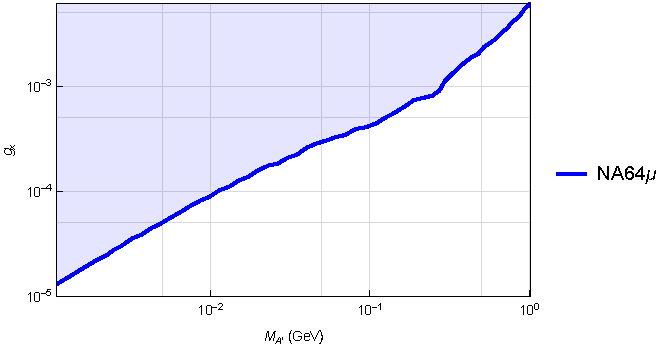
\includegraphics[width=0.6\textwidth]{Constraints picture/NA64mu.pdf}
    \caption{Constraints from NA64$\mu$}
    \label{fig:NA64mu}
\end{figure}

%By LiMing


\subsection{Muon $g-2$}
The muon anomalous magnetic moment is a particularly sharp diagnostic of the Lorentz structure of the new force. The current experimental world average, dominated by the final Fermilab E989 result, is \(a_\mu^{\rm exp}=116592071.5(14.5)\times10^{-11}\). Using the 2025 Muon \(g-2\) Theory Initiative Standard-Model update gives \(\Delta a_\mu\equiv a_\mu^{\rm exp}-a_\mu^{\rm SM} =38(63)\times10^{-11}\)~\cite{Muong-2:2025xyk,Aliberti:2025beg}. This is no longer a robust positive anomaly in the same sense as the older data-driven WP20 comparison~\cite{Aoyama:2020ynm}; therefore we use \((g-2)_\mu\) mainly as a consistency constraint on the axial model.

For a neutral spin-one boson with
\begin{equation}
\mathcal L\supset
A'_\alpha\bar\mu\gamma^\alpha
\left(g_\mu^V-g_\mu^A\gamma_5\right)\mu ,
\end{equation}
the standard one-loop result can be written as~\cite{Leveille:1977rc,Davoudiasl:2014kua,Anastasopoulos:2022ywj}
\begin{equation}
\Delta a_\mu^{A'}=
\frac{m_\mu^2}{4\pi^2m_{A'}^2}
\left[
(g_\mu^V)^2F_V(r)
-(g_\mu^A)^2F_A(r)
\right],
\qquad
r\equiv \frac{m_\mu^2}{m_{A'}^2},
\label{eq:gminus2-vector-axial}
\end{equation}
where
\begin{equation}
F_V(r)=\int_0^1 dx\,
\frac{x^2(1-x)}{1-x+r x^2},
\qquad
F_A(r)=\int_0^1 dx\,
\frac{x(1-x)(4-x)+2r x^3}{1-x+r x^2}.
\label{eq:gminus2-FV-FA}
\end{equation}
The relative minus sign is the main difference from a vector \(L_\mu-L_\tau\) gauge boson. In the heavy-mediator limit,
\begin{equation}
\Delta a_\mu^{A'}\simeq
\frac{m_\mu^2}{12\pi^2m_{A'}^2}
\left[(g_\mu^V)^2-5(g_\mu^A)^2\right],
\qquad m_{A'}\gg m_\mu ,
\label{eq:gminus2-heavy-limit}
\end{equation}
whereas for a light mediator the vector contribution approaches the Schwinger form \(+(g_\mu^V)^2/(8\pi^2)\), while the axial contribution is enhanced by the longitudinal polarization,
\begin{equation}
\Delta a_\mu^{A'}\simeq
\frac{(g_\mu^V)^2}{8\pi^2}
-\frac{(g_\mu^A)^2}{4\pi^2}\frac{m_\mu^2}{m_{A'}^2},
\qquad m_{A'}\ll m_\mu .
\label{eq:gminus2-light-limit}
\end{equation}
In the light-muon mass eigenstate of Eq.~\eqref{eq:light-muon-Apr}, \(g_\mu^V=g_X\sin^2\theta_R\) and \(|g_\mu^A|=g_X\cos^2\theta_R\). Thus the model is dominantly axial and \(\Delta a_\mu^{A'}<0\). If no other new particle contributes, the 2025 comparison roughly requires
\begin{equation}
\Delta a_\mu^{A'} \gtrsim -8.8\times10^{-10}
\quad (2\sigma,\ {\rm WP25}),
\label{eq:gminus2-rough-bound}
\end{equation}
which, in the light-mediator limit, implies the useful estimate
\begin{equation}
g_X\cos^2\theta_R
\lesssim
1.9\times10^{-4}
\left(\frac{m_{A'}}{m_\mu}\right).
\label{eq:gminus2-light-bound}
\end{equation}
This explains why the pure-axial \((g-2)_\mu\) contour in the low-mass region is much stronger than the corresponding vector \(L_\mu-L_\tau\) contour.


%By LiMing
Results: All constraints

\begin{figure}[htbp]
    \centering
    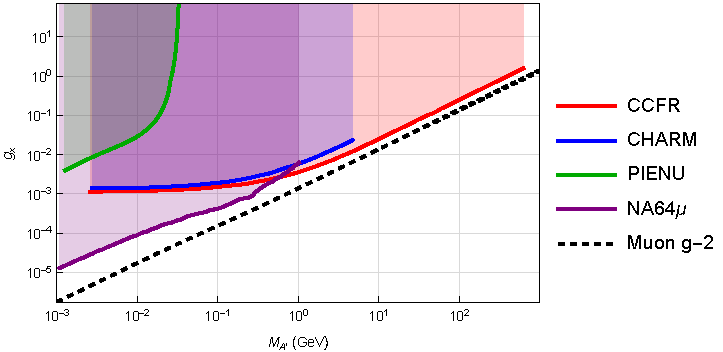
\includegraphics[width=0.6\textwidth]{Constraints picture/AxialConstraints.pdf}
    \caption{Constraints for axial vector model}
    \label{fig:allconstraints}
\end{figure}

%By LiMing

\zb{\subsection{Solar neutrino}

As the axial vector field $A'$ also couples to left-handed neutrinos. The muon- and tau-neutrino currents can also act as source of $A'$~\cite{Fang:2025fvo}. The resulting background field can influence the observed results of the Muon $g-2$ experiment, which enable the current $(g-2)_\mu$ measurement result to be used to constrain the coupling strength. 

We consider solar neutrinos as the dominant source, since they provide the largest neutrino flux at the detector location. The muon- and tau-neutrino components arise through neutrino oscillations during propagation from the Sun to the Earth.
In the relativistic limit, the axial-vector interaction to left-hand neutrinos effectively reduces to a vector-like interaction, such that the neutrino current acts as an electromagnetic-like source which generate a Yukawa potential.
Then, the potential is given by~\cite{Fang:2025fvo},
\begin{equation}
A'^{\alpha} (\vec{x}_d)= \int d^3 x \sum_{\ell = e, \mu, \tau} g_S Q_\ell { \Phi_{\nu_\ell}^{\alpha}(x) }\frac{1}{4 \pi \Delta r}  e^{-m_{A'} \Delta r},
\label{eq:axial-vector-potential}
\end{equation}
where $x_d$ is the position of the detector. $\Phi_{\nu_\ell}^{\alpha}$ is the current of the neutrino $\nu_\ell$, and $\Delta r = |\vec{x}_d - \vec{x}|$ is the distance between the detector and the source. The induced field gives rise to a characteristic sign-changing signal: it is positive during the daytime and negative during the nighttime, superimposed on a small time-independent offset.

In the regime where the interaction range $m^{-1}_{A'}$ is larger than the distance between Sun and Earth, the potential approaches that of a massless mediator, leading to the constraint~\cite{Fang:2025fvo}
\begin{equation}
g_S < 5.8 \times 10^{-18}\  (\text{massless limit}). 
\end{equation}
For larger mediator masses ($m_{A'} > 10^{-17}$ eV), the potential scales as $m^{-2}_{A'}$. The corresponding constraint becomes~\cite{Fang:2025fvo}
\begin{equation}
g_S < 3.1 \times   \frac{ m_{A'}}{{\rm eV}}\ (m_{A'} > 10^{-17}\ \rm{eV}). 
\end{equation}

}

\section{Future Muon Collider Searches}
\label{subsec:muon-collider-angular}

A high-energy muon collider would probe the same muon-philic force in a very different mass range. Ref.~\cite{Huang:2021nkl} studied the ordinary vector \(L_\mu-L_\tau\) gauge boson at a benchmark \(\sqrt{s}=3~{\rm TeV}\) muon collider, using both the two-body process \(\mu^+\mu^-\to\ell^+\ell^-\) and radiative return \(\mu^+\mu^-\to\gamma Z'\). The radiative-return channel is an efficient resonance search for \(m_{A'}<\sqrt{s}\), and in the ultra-relativistic limit its inclusive rate is only mildly sensitive to whether the charged-lepton current is vector or axial. The sharper discriminator for our model is instead the angular distribution in
\begin{equation}
\mu^+\mu^-\to\tau^+\tau^- ,
\end{equation}
where the interference with \(\gamma\) and \(Z\) exchange is chirality dependent.

Neglecting external lepton masses, the unpolarized differential cross section can be written in terms of chiral amplitudes as
\begin{align}
\frac{d\sigma}{d\cos\theta}
&=
\frac{s}{128\pi}
\bigg[
\left(|\mathcal A_{LL}|^2+|\mathcal A_{RR}|^2\right)(1+\cos\theta)^2
\notag\\
&\hspace{2.2cm}
+
\left(|\mathcal A_{LR}|^2+|\mathcal A_{RL}|^2\right)(1-\cos\theta)^2
\bigg],
\label{eq:mucollider-chiral-xsec}
\end{align}
with
\begin{equation}
\mathcal A_{ij}
=
\frac{e^2}{s}
+\frac{g_i^Zg_j^Z}{s-m_Z^2+i m_Z\Gamma_Z}
+\frac{g_i^\mu g_j^\tau}{s-m_{A'}^2+i m_{A'}\Gamma_{A'}} ,
\qquad i,j=L,R .
\label{eq:mucollider-chiral-amplitude}
\end{equation}
For comparison, the ordinary vector and our axial charge assignments are
\begin{equation}
\begin{array}{c|cccc}
&g_L^\mu&g_R^\mu&g_L^\tau&g_R^\tau\\ \hline
{\rm vector} & g'&g'&-g'&-g'\\
{\rm axial} & g_X&-g_X&-g_X&g_X
\end{array}.
\label{eq:mucollider-chiral-couplings}
\end{equation}
This immediately explains why a total-rate reinterpretation of the vector analysis does not capture the main axial effect. Up to a common propagator factor, the photon-\(A'\) interference behaves as
\begin{equation}
\delta_{\gamma A'}^{\rm vector}\propto
-\left[(1+\cos\theta)^2+(1-\cos\theta)^2\right],
\qquad
\delta_{\gamma A'}^{\rm axial}\propto
-(1+\cos\theta)^2+(1-\cos\theta)^2 .
\label{eq:mucollider-interference-pattern}
\end{equation}
The vector case mainly changes the parity-even rate, while the axial case mainly gives a forward--backward distortion. We therefore characterize the effect with
\begin{equation}
A_{\rm FB}=
\frac{\sigma(\cos\theta>0)-\sigma(\cos\theta<0)}
{\sigma(\cos\theta>0)+\sigma(\cos\theta<0)} .
\label{eq:mucollider-afb}
\end{equation}

\begin{figure}[t]
\centering
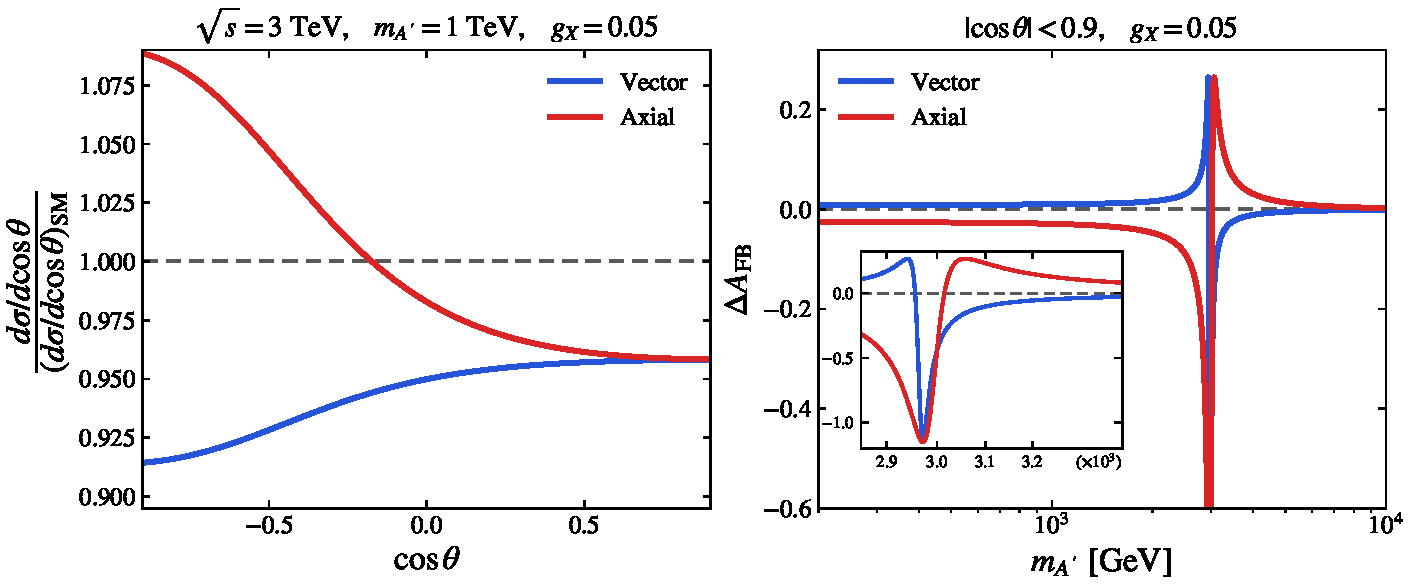
\includegraphics[width=0.94\textwidth]{plots/muon_collider_axial_vector_angular.pdf}
\caption{Future muon-collider angular comparison for \(\mu^+\mu^-\to\tau^+\tau^-\) at \(\sqrt{s}=3~{\rm TeV}\). Left: ratio of the differential cross section to the SM prediction for \(m_{A'}=1~{\rm TeV}\) and \(g'=g_X=0.05\). Right: shift in \(A_{\rm FB}\), integrated over \(|\cos\theta|<0.9\), as a function of \(m_{A'}\). The calculation uses the massless chiral-amplitude formula in Eq.~\eqref{eq:mucollider-chiral-xsec}; the sharp structure near \(m_{A'}\simeq\sqrt{s}\) is the expected \(s\)-channel resonance region.}
\label{fig:muon-collider-angular}
\end{figure}

Fig.~\ref{fig:muon-collider-angular} illustrates the size of the effect. For \(m_{A'}=1~{\rm TeV}\) and \(g_X=0.05\), the vector benchmark changes the \(|\cos\theta|<0.9\) total rate by about \(5\%\), while the axial benchmark changes it by only about \(2\%\). Conversely, the axial case shifts \(A_{\rm FB}\) by \(\Delta A_{\rm FB}\simeq-2.9\times10^{-2}\), larger than the vector shift in this benchmark. A realistic muon-collider limit would therefore require an angular-bin or asymmetry analysis rather than a simple rescaling of the vector \(L_\mu-L_\tau\) contour. This makes the future collider channel complementary to the low-energy probes above: trident, pion-decay, and beam-dump searches constrain the light mediator, whereas a multi-TeV muon collider would test the heavy axial force through parity-odd angular information.

\section{Conclusion}

In this


\section{Acknowledgments}


\bibliographystyle{apsrev4-1}
\bibliography{references}

\end{document}
